\documentclass[10.5pt
%,draft
]{article}


\usepackage{ctex}
\usepackage{graphicx}
\usepackage{amsmath}
\usepackage{xcolor}
\usepackage{physics}
\usepackage{hyperref}
\hypersetup{
    colorlinks=true,
    linkcolor=Blue4Link,
    filecolor=magenta,      
    urlcolor=cyan,
    pdfauthor=徐均益
    }
\definecolor{Blue4Link}{RGB}{46,49,146}
\definecolor{myOrange}{RGB}{178,76,0}
\definecolor{green4eye}{RGB}{0,120,2}%
\definecolor{blue4eye}{RGB}{1,126,218}%
\definecolor{cyan4eye}{RGB}{31,186,190}%
\definecolor{myhighlight}{RGB}{255,214,161}
\definecolor{mybackground}{RGB}{204,232,207}
\usepackage{geometry}
\usepackage{natbib}
\usepackage{subcaption}
\usepackage{epstopdf}
\usepackage{tikz}
\usepackage{psfrag}
\usepackage{natbib}

\def\due{2023 年 5 月 26 日周五 08:40}
\def\Term{2023 年春季}
\def\Course{磁流体力学的数值模拟方法}

\renewcommand{\refname}{参考文献}
\renewcommand{\figurename}{图}
\renewcommand{\abstractname}{摘要}

\title{一维磁流体力学激波 --- 第 4 次作业\footnote{\Term\Course}}

\author{徐均益\footnote{ID: SA22214015 Email: jyxu@mail.ustc.edu.cn}
  \and
  余航\footnote{ID: SA22168021 Email: yh131996@mail.ustc.edu.cn}
  \and
  陈宇韬\footnote{ID: SA22214014 Email: chenyut@mail.ustc.edu.cn}
}

\date{%
\scriptsize%
%CAS Key Laboratory for Basic Plasma Physics, School of Earth and Space Sciences,
%\\
%University of Science and Technology of China, Hefei, Anhui 230026, China
中国科学技术大学核科学技术学院, 合肥 230026 \\
中国科学技术大学物质科学研究院等离子所, 合肥 230026
%
}

\begin{document}

\maketitle

\begin{abstract}
讨论一维磁流体力学 (MHD, Magnetohydrodynamics) 激波问题的有限差分数值解法, 结合理论分析讨论磁声波的特性,
分析数值格式的计算效果, 请在 \textbf{\due}前完成并提交.
\end{abstract}

\section{一维磁流体力学激波\citep{Jeffrey1964}}
守恒型方程
\begin{align}
\frac{\partial U}{\partial t} + \nabla \cdot \boldsymbol{F} &= 0. \label{Eqn:3.1.6}
\end{align}
间断两侧满足关系
\begin{align}
[\tilde{\lambda} U - \boldsymbol{F} \cdot \boldsymbol{n}_1] &= 0 \label{Eqn:3.1.11}
\end{align}
或者
\begin{align}
\tilde{\lambda} [U] &= [\boldsymbol{F} \cdot \boldsymbol{n}_1]. \label{Eqn:3.1.11a}
\end{align}
其中 $\tilde{\lambda}$ 是间断移动的速度, $\boldsymbol{n}_1$ 为间断面的单位法向量.

对一维磁流体, 设所有的物理量只是 $x$ 和 $t$ 的函数,
\begin{align}
U_t + F_x &= 0 \label{Eqn:6.1.1}
\end{align}
这里
\begin{align}
U &= \left[\begin{array}{c}
\rho \\
\rho v_x \\
\frac{1}{2} \rho v^2 + \rho e + p_m \\
\rho v_y \\
H_y \\
\rho v_z \\
H_z
\end{array}\right], \label{Eqn:6.1.2a}
\\
F &= \left[\begin{array}{l}
\rho v_x \\
\rho v_x^2 + p^* \\
v_x \left( \frac{\rho v^2}{2} + \rho e + p_m \right) + v_x p^* - \frac{\mu}{4\pi} H_x \boldsymbol{v} \cdot \boldsymbol{H} \\
\rho v_y v_x - \frac{\mu}{4\pi} H_x H_y \\
H_y v_x - v_y H_x \\
\rho v_z v_x - \frac{\mu}{4\pi} H_x H_z \\
H_z v_x - v_z H_x
\end{array}\right]. \label{Eqn:6.1.2b}
\end{align}
其中 $\rho$, $p$, $e$, $\boldsymbol{v} = (v_x, v_y, v_z)$, 和 $\boldsymbol{H} = (H_x, H_y, H_z)$ 分别是密度, 压强, 内能, 速度, 和磁场. $p_m = \mu H^2/8\pi$ 为磁压, $p^* = p + p_m$ 为总压强. 由磁场无散条件 $\nabla \cdot \boldsymbol{H} = 0$, $H_x$ 是常数, 公式~(\ref{Eqn:3.1.11a}) 因此化为
\begin{align}
\left[ \rho \tilde v_x \right] &= 0 \label{Eqn:6.1.3}
\\
\left[ \rho v_x \tilde v_x + p^* \right] &= 0
\\
\left[\tilde v_x \left( \frac{\rho}{2} v^2 + \rho e + \frac{\mu}{8\pi} H^2 \right) +
v_x p^* -
\frac{\mu}{4\pi} H_x \boldsymbol{v} \cdot \boldsymbol{H} \right] &= 0 \label{Eqn:6.1.6}
\\
\left[ \rho v_y \tilde v_x - \frac{\mu}{4\pi} H_x H_y \right] &= 0
\\
\left[ \tilde v_x H_y - H_x v_y \right] &= 0 \label{Eqn:6.1.8}
\\
\left[ \rho v_z \tilde v_x - \frac{\mu}{4\pi} H_x H_z \right] &= 0
\\
\left[ \tilde v_x H_z - H_x v_z \right] &= 0 \label{Eqn:6.1.10}
\end{align}
此处 $\tilde v_x$ 相对于间断流体速度的 $x$ 分量, 即
\begin{align}
\tilde v_x = v_x - \tilde\lambda
\end{align}
假设 $\tilde\lambda$ 为常数. 使用随间断运动的坐标系,
在这个坐标系中速度 $\boldsymbol{v}' = (v_x', v_y', v_z')$, 磁场 $\boldsymbol{H'} = (H_x', H_y',
H_z')$. Galilean 变换的结果是 $\boldsymbol{H}$ 不变, 速度由下面方程决定
\begin{align*}
v_x' = & v_x - \tilde\lambda = \tilde v_x \\
v_y' = & v_y \\
v_z' = & v_z. 
\end{align*}
在不造成混淆的情况下, 直接用 $\boldsymbol{v} = (v_x, v_y, v_z)$ 和 $\boldsymbol{H} = (H_x, H_y, H_z)$ 表示 ${\bf
v'}$ 和 $\boldsymbol{H}'$. 将间断位置设为坐标原点, 即
\begin{align*}
x &= 0.
\end{align*}
定义
\begin{align*}
\left<Q\right> &= \frac{1}{2}(Q_0 + Q_1),
\end{align*}
角标 0 和 1 分别表示间断两侧 (波前/上游和波后/下游) 的量. 进而可以将跃变关系~(\ref{Eqn:6.1.3})-(\ref{Eqn:6.1.10}) 表示为
\begin{align}
m[\tau] - [v_x] &= 0 \label{Eqn:6.1.4a}
\\
m[v_x] + [p] + \frac{\mu}{4\pi} \left< \bf H \right> \cdot [\bf H ] &=
0\label{Eqn:6.1.5a}
\\
m[v_y] - \frac{\mu}{4\pi} H_x [H_y] &= 0\label{Eqn:6.1.7a}
\\
m \left<\tau \right> [H_y] + \left< H_y \right> [v_x] - H_x [v_y] &= 0\label{Eqn:6.1.8a}
\\
m [v_z] - \frac{\mu}{4\pi} H_x [H_z] &= 0
\\
m \left< \tau \right> [H_z] - H_x [v_z] &= 0\label{Eqn:6.1.10a}
\end{align}
这里 
\begin{align}
  \tau &= \rho^{-1},
  \\
  m &= \rho_1 \tilde v_{x1} = \rho_0 \tilde v_{x0}.
\end{align}
同时选取坐标系使得 $\left< H_z \right> = 0$. 这样, 很容易得到关于 $m$
(或者激波速度 $\tilde\lambda$) 的方程 (力学关系), 快慢磁声激波情况下为
\begin{align}
(m^2 + [\tau]^{-1}[p]) \left( m^2 - \left<\tau\right>^{-1} \frac{\mu H_x^2}{4\pi} \right)
&= m^2 \left<\tau\right>^{-1} \frac{\mu}{4\pi}
\left<H_y\right>^2\label{Eqn:6.1.13}
\end{align}
横波 (Alfven 波) 情况下为,
\begin{align}
\left<\tau\right> m^2 - \frac{\mu H_x^2}{4\pi} = 0.\label{Eqn:6.1.14}
\end{align}
能量方程~(\ref{Eqn:6.1.6}) 可以改写为,
\begin{align}
m \Bigg\{ \left[ e + \frac{\mu}{8\pi} \tau H^2 \right] +& [\tau] \left( \left<p\right>
+
\frac{\mu}{8\pi} \left<\bf H_t^2\right> - \frac{\mu}{8\pi} H_x^2 \right)
\nonumber\\
-& \frac{\mu}{4\pi} [\tau \bf H_t] \cdot \left< \boldsymbol{H}_t \right> \Bigg\} = 0
\end{align}
此处 $\boldsymbol{H}_t$ 是横向磁场
\begin{eqnarray*}
\boldsymbol{H}_t = \boldsymbol{H} - (\boldsymbol{H} \cdot \boldsymbol{n}_1) \boldsymbol{n}_1.
\end{eqnarray*}
最后得到
\begin{align}
m = 0\label{Eqn:6.1.6aa}
\end{align}
或
\begin{align}
[e] + \left<p\right>[\tau] = -\frac{\mu}{16\pi} [\tau][\bf H_t]^2.\label{Eqn:6.1.6ba}
\end{align}
(\ref{Eqn:6.1.6ba}) 称为广义 Rankine-Hugoniot 关系. (\ref{Eqn:6.1.6aa}) 为接触间断条件.

结合方程~(\ref{Eqn:6.1.13}), (\ref{Eqn:6.1.14}) 和 (\ref{Eqn:6.1.6aa}),
将磁流体力学间断分为快慢激波, 横向间断(激波)和接触间断.

不失一般性, 我们可以选取坐标系使得激波前 $H_x > 0$, $H_{y0} > 0$, 且假定 $x$ 轴指向 $\boldsymbol{n}$ 的正方向, $\boldsymbol{n}$ 为激波前指向激波后的单位向量,
即流体流入的方向. 整理后, 可将快慢磁声激波关系表示为
\begin{align}
\bar{\eta} &= h\left\{\frac{-\frac{1}{2}\gamma h \sin\theta_0 -
(1-s_0) \pm
\sqrt{R(h)}}{2 s_0 \sin\theta_0 - (\gamma-1) h}\right\},\label{Eqn:6.2.15}
\\
\bar{Y} &= \frac{\gamma}{s_0} \left\{-\frac{1}{2} h^2 +
h\left(\frac{\frac{1}{2}\gamma h \sin\theta_0 - (1-s_0) \pm
\sqrt{R(h)}}{2 s_0 \sin\theta_0 - (\gamma-1) h}\right)\right\}\label{Eqn:6.2.16a}
\\
&= \frac{\gamma}{s_0} \left\{-\frac{1}{2} h^2 +
h\left(\frac{\bar{\eta}/h - \sin\theta_0}{1 - (\bar{\eta}/h)
\sin\theta_0}\right)\right\},\label{Eqn:6.2.16b}
\end{align}
$\bar{\eta}$, $\eta$. $h$, $\bar{Y}$, $\theta_0$, $s_0$ 和 $R$ 的定义如下,
\begin{align}
\bar{\eta} &= \frac{[\rho]}{\rho_0}, \qquad \eta = \frac{\rho_1}{\rho_0} = 1 + \bar{\eta} \nonumber\\
h &= \frac{[H_y]}{H_0}, \qquad H_j = \sqrt{H_x^2+H_{yj}^2} \qquad (j=0,1) \nonumber\\
\bar{Y} &= \frac{[p]}{p_0}, \qquad Y = \frac{p_1}{p_0} = 1 + \bar{Y} \nonumber\\
s_j &= \frac{\gamma p_j}{(\mu/4\pi)H_j^2} \qquad (j=0,1) \nonumber\\
\sin\theta_j &= \frac{H_{yj}}{H_j}, \qquad 0^\circ < \theta_j < 90^\circ \qquad (j=0,1) \nonumber\\
R(h) &= h^2[\frac{1}{4} \gamma^2 \sin^2\theta_0 - (\gamma-1)] + h\sin\theta_0
(2-\gamma)(1+s_0)
\nonumber\\
& \quad + 4s_0 \sin^2\theta_0 + (1-s_0)^2.\label{Eqn:6.2.17}
\end{align}
此外
\begin{equation}
\frac{\tilde{v}_{x1}}{b_{x1}} = \eta^{\frac{1}{2}} \frac{\tilde{v}_{x0}}{b_{x0}} =
\frac{1}{[1-(\bar{\eta}/h) \sin\theta_0]^{1/2}}
\end{equation}
从而可以直接求得激波速度 $\tilde{\lambda}$ ($=v_{x0}-\tilde{v}_{x0}$).

$[v_y]$ 表示为
\begin{align}\label{Eqn:6.2.18a}
\frac{[v_y]}{b_{x1}} = \frac{b_{x1} h}{\tilde{v}_{x1} \cos\theta_0} =
\frac{h}{\cos\theta_0} \left[1 - \left(\frac{\bar{\eta}}{h}\right)
\sin\theta_0\right]^{1/2}.
\end{align}
给定 $h$ 和激波前状态, 我们可以确定激波速度以及激波后的态. 用 $v_n$, $\tilde{v}_n$ 和 $H_n$ 取代 $v_x$, $\tilde v_x$ 和 $H_x$,
可以得到不依赖于 $x$ 轴选择的一般形式. 对于 (1 型) 快磁声激波和慢激波, 激波上下游的关系式如下文所述.

\subsection{1 型快激波}
\begin{align}
h_f &= \frac{[H_y]}{H_0}
\\
s_0 &\ge 1 - \frac{\gamma}{\gamma-1} \sin^2\theta_0, \quad 0 < h_f \le \hat{\hat{h}}_f
\quad \left(\hat{\hat{h}}_f = \frac{2}{\gamma-1} \sin\theta_0\right)
\\
\bar{\eta}_f &= h_f \left\{\frac{-\frac{1}{2} \gamma h_f \sin\theta_0 - (1-s_0) +
\sqrt{R(h_f)}}{2s_0 \sin\theta_0 - (\gamma-1) h_f}\right\}, \nonumber\\
& \qquad \bar{\eta}_{f\max} = \frac{2}{\gamma-1}
\\
\bar{Y}_f &= \frac{\gamma}{s_0} \left\{-\frac{1}{2} h_f^2 + h_f \frac{-\frac{1}{2}
\gamma h_f \sin\theta_0 - (1-s_0) + \sqrt{R(h_f)}}{2s_0 \sin\theta_0 - (\gamma-1)
h_f}\right\}, \nonumber
\\
&= \frac{\gamma}{s_0} \left\{-\frac{1}{2} h_f^2 + h_f \frac{(\bar{\eta}_f/h_f) -
\sin\theta_0}{1 - (\bar{\eta}_f/h_f)\sin\theta_0}\right\}, \quad \bar{Y}_{f\max} = \infty
\\
\frac{\tilde{v}_{n1}^f}{b_{n1}^f} &= \eta_f^{-1/2} \frac{\tilde{v}_{n0}^f}{b_{n0}^f} =
\frac{1}{[1 - (\bar{\eta}_f/h_f) \sin\theta_0]^{1/2}}
\\
\frac{[v_n^f]}{b_{n1}^f} &= - \bar{\eta}_f \frac{\tilde{v}_{n1}^f}{b_{n1}^f} =
-\frac{\bar{\eta}}{[1 - (\bar{\eta}_f/h_f) \sin\theta_0]^{1/2}}
\\
\frac{[v_y^f]}{b_{n1}^f} &= \frac{b_{n1}^f}{\tilde{v}_{n1}^f} \frac{h_f}{\cos\theta_0}
= \frac{h_f}{\cos\theta_0} \left[1 - \left(\frac{\bar{\eta}_f}{h_f}\right)
\sin\theta_0\right]^{1/2}
\\
R(h_f) &= h_f^2 \left[\frac{1}{4} \gamma^2 \sin^2\theta_0 - (\gamma - 1)\right] + h_f
\sin\theta_0 (2 - \gamma) (1 + s_0)
\nonumber\\
& \quad + 4s_0 \sin^2\theta_0 + (1 - s_0)^2
\end{align}

\subsection{慢激波}
\begin{align}
h_s &= -\frac{[H_y]}{H_0}, \quad 0 \le h_s \le \sin\theta_0 \quad (0 < \theta_0 < 90^\circ)
\\
\bar{\eta}_s &= h_s \left\{\frac{(1-s_0) - \frac{1}{2} \gamma h_s \sin\theta_0 +
\sqrt{R^+ (h_s)}}{(\gamma-1) h_s + 2 s_0 \sin\theta_0}\right\}
\\
\bar{Y}_s &= \frac{\gamma}{s_0} \left\{-\frac{h_s^2}{2} + h_s \left[\frac{(1-s_0) +
\frac{1}{2} \gamma h_s \sin\theta_0 + \sqrt{R^+ (h_s)}}{(\gamma-1) h_s + 2
\sin\theta_0}\right]\right\}
\\
\frac{\tilde{v}_{n1}^s}{b_{n1}^s} &= \frac{1}{\eta_s^{1/2}}
\frac{\tilde{v}_{n0}^s}{b_{n0}^s} = \frac{1}{[1+(\bar{\eta}_s/h_s)\sin\theta_0]^{1/2}}
\\
\frac{[v_n^s]}{b_{n1}^s} &= - \bar{\eta}_s \frac{\tilde{v}_{n1}^s}{b_{n1}^s} =
-\frac{\bar{\eta}_s}{[1+(\bar{\eta}_s/h_s)\sin\theta_0]^{1/2}}
\\
\frac{[v_y^s]}{b_{n1}^s} &= - \frac{b_{n1}^s}{\tilde{v}_{n1}^s}
\frac{h_s}{\cos\theta_0} = -\frac{h_s}{\cos\theta_0}
[1+(\bar{\eta}_s/h_s)\sin\theta_0]^{1/2}
\\
R^+(h_s) &= h_s^2 [\frac{1}{4} \gamma^2 \sin^2\theta_0 - (\gamma-1)] - h_s \sin\theta_0
(2-\gamma)(1+s_0) \nonumber
\\
& \quad + 4s_0 \sin^2\theta_0 + (1-s_0)^2
\end{align}

\section{数值实验}

考虑下列初值问题
\begin{align}
U(x,t)|_{t=0} = \left\{ \begin{array}{ll}
U_L, & \quad x < x_0 \\
U_R, & \quad x > x_0
\end{array} \right.
\end{align}
或者
\begin{align}
W(x,t)|_{t=0} = \left\{ \begin{array}{ll}
W_L, & \quad x < x_0 \\
W_R, & \quad x > x_0
\end{array} \right.
\end{align}
的有限差分数值计算. 这里 $U$ 的表达式由方程~(\ref{Eqn:6.1.2a}) 给出, 而
\begin{align}
W = \left[ \begin{array}{ccccccc}
\rho,
p,
v_x,
v_y,
v_z,
H_y,
H_z
\end{array} \right]^T.
\end{align}
上标 $T$ 表示转置操作. 取 $\gamma=5/3$, $\mu=1$, $H_x=5$. 分别就下面两种初值条件,
设计有限差分格式进行数值求解并作图讨论结果.

\subsection{较弱的快慢激波}
取 $x_0 = 0.0$, 快激波条件为
\begin{align}
W_L &= \left[\begin{array}{cccccc}
2.121,
4.981,
-13.27,
-0.163,
-0.6521,
2.572,
10.29
\end{array}\right]^T,
\nonumber\\
W_R &= \left[\begin{array}{ccccccc}
1,
1,
-15.3,
0,
0,
1,
4
\end{array}\right]^T. \label{Eqn:WFast}
\end{align}
慢激波条件为
\begin{align}
W_L &= \left[\begin{array}{ccccccc}
2.219,
0.4442,
0.5048,
0.0961,
0.0961,
1,
1
\end{array}\right]^T,
\nonumber\\
W_R &= \left[\begin{array}{ccccccc}
1,
0.1,
-0.9225,
0,
0,
1,
1
\end{array}\right]^T.
\end{align}
其中快激波的计算结果如图~\ref{Fig:WFast} 所示.
\begin{figure}
\begin{center}
\begin{tabular}{cc}
\includegraphics[width=.45\textwidth]{WFast077.eps} &
\includegraphics[width=.45\textwidth]{WFast261.eps}
\\
(a) & (b)
\end{tabular}
\caption{初值条件~(\ref{Eqn:WFast}) 情况下的快激波在 $t = 0.1$ 时的 TVD 格式 \citep{vanLeer1974,Harten1983} 计算结果. 从上到下数据为无量纲形式的密度, 能量, 质量流和磁场垂直分量.
  (a) 网格数为 133; (b) 网格数为 261.} \label{Fig:WFast}
\end{center}
\end{figure}

\subsection{一维 MHD 快激波 (Mach 数为 10)\citep{Dai1994}}
取 $x_0 = 0.2$, 快磁声激波的初值条件为\footnote{
  根据附件 Excel 表计算得到, 和文献 \citet{Dai1994} 稍有出入.
}
\begin{align}
W_L &= \left[\begin{array}{cccccc}
3.896,
305.9,
0,
-0.058,
-0.226,
3.951,
15.8
\end{array}\right]^T,
\nonumber\\
W_R &= \left[\begin{array}{ccccccc}
1,
1,
-15.3,
0,
0,
1,
4
\end{array}\right]^T.\label{Eqn:Fast}
\end{align}
作为参考, 使用 TVD (Total Variance Diminishing) 格式 \citep{vanLeer1974,Harten1983} 的数值计算结果如图~\ref{Fig:Fast} 所示.
\begin{figure}
\begin{center}
\includegraphics[height=.78\textwidth]{FShockNum.eps}
\caption{初值条件 ~(\ref{Eqn:Fast}) 情况下快激波的 TVD 格式 \citep{vanLeer1974,Harten1983} 对应于 $t=0$, 0.05 和 0.1 时的计算结果.}\label{Fig:Fast}
\end{center}
\end{figure}

\subsection{一维 MHD 慢激波 (Mach 数为 3.5)\citep{Dai1994}}
同样取 $x_0 = 0.2$, 慢磁声激波的初值条件为
\begin{align}
W_L &= \left[\begin{array}{ccccccc}
3.108,
1.4336,
0,
0.2633,
0.2633,
0.1,
0.1
\end{array}\right]^T,
\nonumber\\
W_R &= \left[\begin{array}{ccccccc}
1,
0.1,
-0.9225,
0,
0,
1,
1
\end{array}\right]^T.\label{Eqn:Slow}
\end{align}
作为参考, 使用 TVD 格式 \citep{vanLeer1974,Harten1983} 的数值计算结果如图~\ref{Fig:Slow} 所示.
\begin{figure}
\begin{center}
\includegraphics[height=.78\textwidth]{SShockNum.eps}
\caption{初值条件~(\ref{Eqn:Slow}) 情况下慢激波的 TVD 格式 \citep{vanLeer1974,Harten1983} 对应于 $t=0$, 0.8 和 1.6 时计算结果.}\label{Fig:Slow}
\end{center}
\end{figure}

附件 Excel 表给出用激波关系计算的上下游变量值. 表 Dai1994 为依据文献 \citet{Dai1994} 给出的初值, 表 FnS 是简单地复制表 Dai1994 并改变单元 D2, N2 得到的另一组初值,
此时红色部分的数据没有用处. 其中, B-D, F-H 列为快激波数据, L-M, P-R 列为慢激波数据. 蓝色区域为输入, 红色数据为文献 \citet{Dai1994} 中的数据 (可能有误), B-D 和 L-M 为
Gauss 单位制数值, F-H, P-R 为无量纲单位数值 (具体方程和说明见第 \ref{DLess} 节), C28, G28 为快激波速度 (正方向定义为上游指向下游, 负值表示从下游指向上游, 即向右传播),
M28, Q28 为慢激波速度 (负值同样表示下游向上游传播).

\textbf{后面两个激波较强, 特别是快激波, 如果觉得数值计算上有困难, 可以只完成前面较弱激波的计算.}

\section{分工说明}

郑惠南提供了最初的报告文本, 数值计算结果生成的图形文件. 高新亮对整个文档结构, 规范, 文件清单进行了检查, 确认.

\section{无量纲守恒形式方程}\label{DLess}
如果要使用无量纲数值, 可以将磁流体力学方程表示为
\begin{align}
\frac{\partial U}{\partial t} + \frac{\partial F}{\partial x} = 0 \label{Eqn:MHD}
\end{align}
其中
\begin{align}
U = & \left[ \begin{array}{l}
\rho\\
\rho v^2 + H_y^2 + H_z^2 + \frac{\beta p}{\gamma -1}
\\
\rho v_x\\
\rho v_y\\
\rho v_z\\
H_y\\
H_z
\end{array} \right], \\
F = & \left[ \begin{array}{l}
\rho v_x\\
\rho v_x \left(v^2 + \frac{\gamma}{\gamma - 1} \frac{\beta p}{\rho} \right) + 2(H_y^2 v_x + H_z^2 v_x - H_x H_y v_y - H_x H_z v_z)
\\
\rho v_x^2 + \frac{\beta}{2} p + \frac{1}{2} (H_y^2 + H_z^2)\\
\rho v_x v_y - H_x H_y\\
\rho v_x v_z - H_x H_z\\
v_x H_y - v_y H_x\\
v_x H_z - v_z H_x
\end{array} \right] \label{Eqn:Flux}
\end{align}
这里 $v^2 = v_x^2 + v_y^2 + v_z^2$. 若取 $\rho_0 = 1$, $p_0 = 1$, $v_0 = 1$, $H_0 = 1/\sqrt{4\pi}$, 则 $\beta = 2$.

\subsection{\textit{Lax-Wendroff}格式}
\textit{Lax-Wendroff}格式适用于守恒型方程
\begin{align}
\frac{\partial \vb w}{\partial t} + \frac{\partial \vb F}{\partial x} = 0
\end{align}
其中差分格式为
\begin{align}
u_j^{n+1} =& u_j^n - \frac{\Delta t}{2\Delta x} (F_{j+1}^n - F_{j-1}^n) \nonumber\\
& + \frac{\Delta t^2}{2\Delta x^2} \left[A_{j+1/2}^n (F_{j+1}^n-F_j^n) - A_{j-1/2}^n (F_j^n -
F_{j-1}^n)\right]
\end{align}
其中 $A = \frac{\partial F}{\partial u}$, $A$ 的表达式为
\begin{equation}
   \mqty[
0  &  0  &  1  &  0  &  0  &  0  &  0 \\
% (2 H_x \rho (H_y m_y+H_z m_z)+m_x (\rho (-\gamma E +(\gamma-2) H_y^2+(\gamma-2) H_z^2)+2 (\gamma-1) m_y^2+2 (\gamma-1) m_z^2)+2 (\gamma-1) m_x^3)/\rho^3  &  (\gamma m_x)/\rho  &  -((-\gamma E \rho+(\gamma-2) H_y^2 \rho+(\gamma-2) H_z^2 \rho+3 (\gamma-1) m_x^2+(\gamma-1) m_y^2+(\gamma-1) m_z^2)/\rho^2)  &  -((2 (H_x H_y \rho+(\gamma-1) m_x m_y))/\rho^2)  &  -((2 (H_x H_z \rho+(\gamma-1) m_x m_z))/\rho^2)  &  -((2 (H_x m_y+(\gamma-2) H_y m_x))/\rho)  &  -((2 (H_x m_z+(\gamma-2) H_z m_x))/\rho) \\
\dots  &  \dots  &  \dots  &  \dots  &  \dots  &  \dots  &  \dots \\
\frac{(\gamma-1) v^2-2v_x^2}{2 }  &  \frac{\gamma-1}{2}  &  (3-\gamma) v_x  & (1-\gamma) v_y  &  (1-\gamma) v_z  &  (2-\gamma) H_y  &  (2-\gamma) H_z \\
-v_x v_y  &  0  &  v_y  &  v_x  &  0  &  -H_x  &  0 \\
-v_x v_z  &  0  &  v_z  &  0  &  v_x  &  0  &  -H_x \\
\frac{H_x v_y-H_y v_x}{\rho}  &  0  &  \frac{H_y}{\rho}  &  -\frac{H_x}{\rho}  &  0  &  v_x  &  0 \\
H_x v_z-H_z v_x  &  0  &  \frac{H_z}{\rho}  &  0  &  -\frac{H_x}{\rho}  &  0  &  v_x ]
\end{equation}
矩阵第二行7个元素分别为
\begin{subequations}
	\begin{gather}
% (2 H_x \rho (H_y m_y+H_z m_z)+m_x (\rho (-\gamma E +(\gamma-2) H_y^2+(\gamma-2) H_z^2)+2 (\gamma-1) m_y^2+2 (\gamma-1) m_z^2)+2 (\gamma-1) m_x^3)/\rho^3   \\
-\frac{2 (H_y^2+H_z^2) v_x (1- \gamma) -2 H_x (H_y v_y+H_z v_z )(1 - \gamma) - p v_x \beta \gamma + v_x v^2 (2 - 3 \gamma + \gamma^2) \rho}{(1 - \gamma) \rho}\\
  \gamma v_x   \\
  -((-\gamma E \rho+(\gamma-2) H_y^2 \rho+(\gamma-2) H_z^2 \rho+3 (\gamma-1) m_x^2+(\gamma-1) m_y^2+(\gamma-1) m_z^2)/\rho^2)   \\
  -((2 (H_x H_y \rho+(\gamma-1) m_x m_y))/\rho^2)   \\
  -((2 (H_x H_z \rho+(\gamma-1) m_x m_z))/\rho^2)   \\
  -((2 (H_x m_y+(\gamma-2) H_y m_x))/\rho)   \\
  -((2 (H_x m_z+(\gamma-2) H_z m_x))/\rho) 
\end{gather}
\end{subequations}
其中
$ m_x = \rho v_x,
m_y = \rho v_y,
m_z = \rho v_z.$
单元边界上的值可以取
\begin{align}
A_{j \pm 1/2}^n = A(u_{j \pm 1/2}^n), \qquad u_{j \pm 1/2}^n = \frac{1}{2} (u_j^n + u_{j \pm 1}^n)
\end{align}
\section{附件}
\begin{enumerate}
\item
assign4.tex--本报告 \LaTeX 源文件
\item
assign4.pdf--本报告 PDF (Portable Document Format) 输出文件
\item
References.bib -- 文献文件
\item
WFast077.eps--初值条件 (\ref{Eqn:WFast}) 情况下的快激波数值结果 (TVD 格式), 133网格, 对应图~\ref{Fig:WFast} (a)
\item
WFast261.eps--初值条件 (\ref{Eqn:WFast}) 情况下的快激波数值结果 (TVD 格式), 261网格, 对应图~\ref{Fig:WFast} (b)
\item
FShockNum.eps--初值条件 (\ref{Eqn:Fast}) 情况下 (快磁声激波) 数值计算得到的物理量各时刻图形 (TVD 格式), 对应图~\ref{Fig:Fast}
\item
SShockNum.eps--初值条件 (\ref{Eqn:Slow}) 情况下 (慢磁声激波) 数值计算得到的物理量各时刻图形 (TVD 格式), 对应图~\ref{Fig:Slow}
\item
MHDShock.xlsx -- 快慢激波两侧态分析的 EXCEL 表格文件
\end{enumerate}

% 以下两行是中文文献国家标准的格式, 如果安装了这两个格式, 建议使用它们
\bibliographystyle{gbt7714-author-year}
% \bibliographystyle{gbt7714-numerical}
%

\bibliography{References}

\end{document}
